\documentclass[serif,mathserif, 12pt]{beamer}
\usepackage{etex}
\usepackage{amsmath, amsfonts, epsfig, xspace}
\usepackage{algorithm,algorithmic}
\usepackage{pstricks,pst-node}
\usepackage{multimedia}
\usepackage[normal,tight,center]{subfigure}
\setlength{\subfigcapskip}{-.5em}
\usepackage{tkz-euclide}
\usetkzobj{all}
\usepackage{beamerthemesplit}
\usetheme{lankton-keynote}
\usepackage{graphicx,color}
% remove caption of figure
\usepackage[labelformat=empty]{caption}

\usepackage[none]{hyphenat} % hyphenation is ugly in slides
\usepackage{parskip}

\usepackage{relsize} % \smaller to change size

\usepackage{tikz}
\usetikzlibrary{calc}

\usetikzlibrary{arrows}

\newcommand{\TikzDraw}[2][]{
  \begin{tikzpicture}[overlay, remember picture, shift={(current page.center)}, #1]
    #2
  \end{tikzpicture}
}

\newcommand{\gridlines}{
  \TikzDraw{
    \draw[help lines,xstep=.2,ystep=.2,red!20] (current page.south west) grid (current page.north east);
    \draw[help lines,xstep=1,ystep=1,red] (current page.south west) grid (current page.north east);
    \foreach \x in {-15,-14,...,15} {
      \node [anchor=north, red] at (\x,0) {\tiny \x};
      \node [anchor=east,red] at (0,\x) {\tiny \x};
    }
  }
}

\newcommand{\DrawOnImg}[3][]
{
  \begin{tikzpicture}
    \node[anchor=south west,inner sep=0] (image) at (0,0){
      #2
    };
    \begin{scope}[x={(image.south east)},y={(image.north west)}]
      \ifthenelse{\equal{#1}{grid}}
                 {\draw[color=blue, style=dashed] (0,0) grid[xstep=.1, ystep=.1] (1.0001,1.0001);}
                 {}
                 #3
    \end{scope}
  \end{tikzpicture}
}

\usetikzlibrary{matrix}

\newcommand{\BOLD}[1]{\mathbf{#1}}
\newcommand{\BOLDG}[1]{\boldsymbol{#1}}
\newcommand{\PDIF}[2]{\frac{\partial #1}{\partial #2}}
\newcommand{\TODO}[1]{\textcolor{red}{#1}}
\newcommand{\TODOB}[1]{\textcolor{blue}{#1}}
\newcommand{\TODOG}[1]{\textcolor{green!50!black}{#1}}
\newcommand{\argmin}{\operatornamewithlimits{arg\min}}
\DeclareMathOperator{\tr}{tr}
\DeclareMathOperator{\cond}{cond}
\DeclareMathOperator{\ST}{s.t.}
\DeclareMathOperator{\diag}{diag}
\DeclareMathOperator{\Div}{div}

\title[\hspace{2em}\insertframenumber/\inserttotalframenumber]{Fast and Deep Deformation Approximations}
\date{3th, July 2018}

\author{Stephen W. Bailey, Dave Otte, \\Paul Dilorenzo, James F. O'Brien}

\makeatletter
\let\@@magyar@captionfix\relax
\makeatother

\begin{document}

\maketitle

\begin{frame}
  \frametitle{Background}
  \begin{itemize}
  \item Character rigs.
    \pause
  \item \TODOG{Film quality rigs, realistic deformation}
  \item \TODO{Real time rigs, fast computation}
  \end{itemize}
  \TikzDraw {
    \visible<2> {
    \node at (-2.5, -2.3) {
      \includegraphics[width=0.4\textwidth]{img/hulk1}
    };
    \node at (2.5, -2.3) {
      \includegraphics[width=0.41\textwidth]{img/hulk2}
    };
    }
  }
\end{frame}

\begin{frame}
  \frametitle{Goal}
  \begin{itemize}
  \item Evaluate \textbf{\TODOG{film-quality}} rigs in \textbf{\TODO{real time}}.
  \end{itemize}
\end{frame}

\begin{frame}
  \frametitle{Ideas}
  \begin{itemize}
  \item Motion decomposition
    \[
    \text{Deformation} = \text{Linear portion} + \text{Nonlinear portion}
    \]
  \pause
  \item For \emph{nonlinear portion}:
    \begin{itemize}
    \item[-] Traditional approach: pose-space, cage-based, physically-based...
      \pause
    \item[-] This paper: \TODO{neural network}.
    \end{itemize}
  \end{itemize}
\end{frame}

\begin{frame}
  \frametitle{Pipeline}
  \begin{figure}
    \centering
    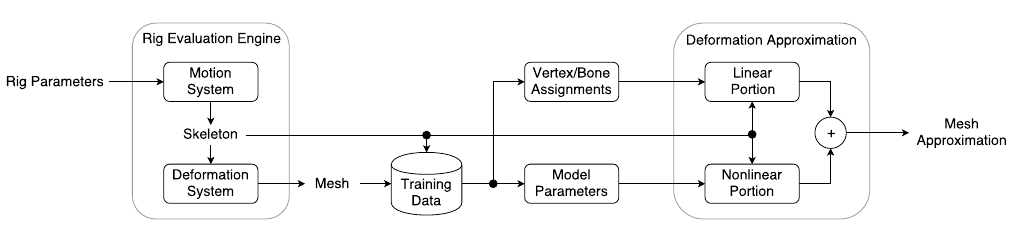
\includegraphics[width=\textwidth]{img/pipeline}
  \end{figure}
\end{frame}

\begin{frame}
  \frametitle{Rig Function}
  \begin{itemize}
  \item Rig function $r(p)=(d\circ m)(p)$
  \item Skeletal motion $S = m(p)$
    \[
    \begin{split}
    &S = [X_1, t_1, X_2, t_2, \dots, X_m, t_m], \\
    &X_i \in R^{3\times 3}, t_i \in R^3
    \end{split}
    \]
  \item Mesh deformation $V = d(S)$
  \end{itemize}
  \TikzDraw {
    \visible<2> {
      \node at (0, -2.5) {\TODO{\textbf{Approximate $d(S)$}}};
    }
  }
\end{frame}

\begin{frame}
  \frametitle{Deformation Approximation}
  \begin{itemize}
  \item Linear Skinning: for vertex $k$ assigned to bone $b_k$
    \begin{equation*}
      \hat d_k(S) = X_{b_k}(X_{b_k}^0)^{-1}(v_k^0-t_{b_k}^0)+t_{b_k}
    \end{equation*}
  \end{itemize}
  \TikzDraw {
    \node at (0, -2.) {
      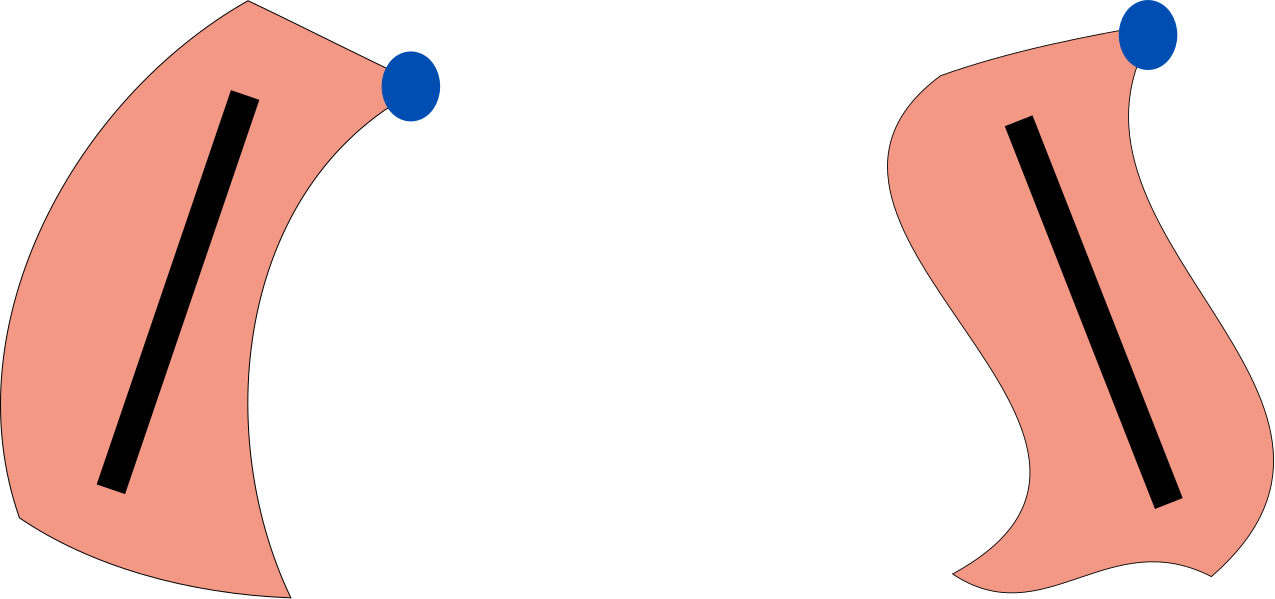
\includegraphics[width=0.6\textwidth]{img/linear_skinning}
    };
    \node at (-1.5, -2.2) {$(X_{b_k}^0, t_{b_k}^0)$};
    \node at (-0.8, -1) {$v_k^0$};
    \node at (3.3, -2.2) {$(X_{b_k}, t_{b_k})$};
    \node at (3.2, -0.8) {$\hat d_k(S)$};
  }
\end{frame}

\begin{frame}
  \frametitle{Deformation Approximation}
  \begin{itemize}
  \item Nonlinear deformation
    \begin{itemize}
    \item[-] Residual $d(S)-\hat d(S)$, \TODO{in terms of global coordinate system.}
      \TikzDraw {
        \node at (-5, 1) {
          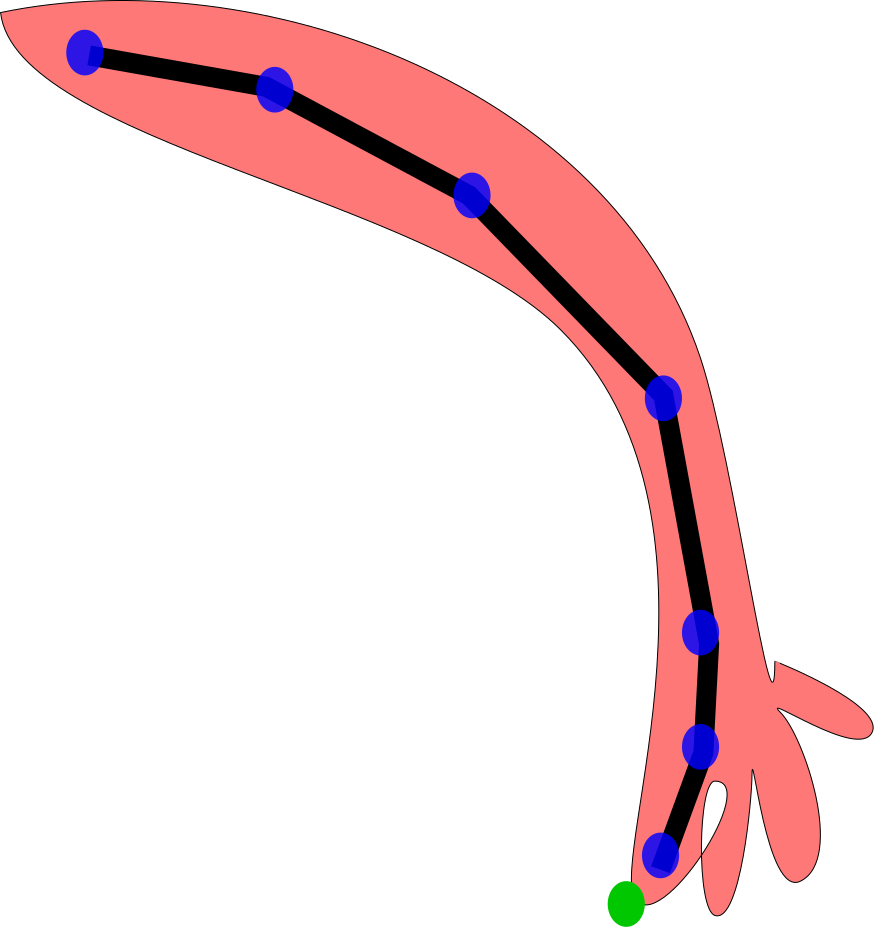
\includegraphics[width=0.2\textwidth]{img/hand}
        };
      }
      \pause
    \item[-] Express residual in local frame
      \[
      f_k(S) = (X_{b_k})^{-1}(d_k(S)-t_{b_k}) - (X_{b_k}^0)^{-1}(v_k^0-t_{b_k}^0)
      \]
      \pause
    \item[-] Deformation function
      \[
      d_k(S) = X_{b_k}\left((X_{b_k}^0)^{-1}(v_k^0-t_{b_k}^0)+\TODO{f_k(S)}\right) + t_{b_k}
      \]
    \end{itemize}
  \end{itemize}
  \TikzDraw {
    \visible<4-> {
      \node at (0, -3.2) {\TODO{$f_k(S) \approx n_k(S; \theta)$ }};
    }
  }
\end{frame}

\begin{frame}
  \frametitle{Deformation Approximation}
  \begin{itemize}
  \item Deformation approximation
    \begin{equation*}
      \tilde d_k(S; \theta) = \hat d_k(S) + X_{b_k}n_k(S; \theta)
    \end{equation*}
  \item Training problem over $n$ examples
    \[
    \hat \theta_k  = \argmin_{\theta} \sum_{i=1}^n\|d_k(S^i)-\tilde d_k(S^i; \theta)\|^2, \forall k
    \]
  \end{itemize}
  \TikzDraw {
    \visible<2> {
      \node at (0, -2.5) {
        \TODO{$\hat \theta_k \rightarrow \theta_{P_j=\{k|b_k=j\}}$}
      };
    }
  }
\end{frame}

\begin{frame}
  \frametitle{Technical Details}
  \begin{itemize}
  \item Network structure: 2 fully connected hidden layers + 1 dense output layer
  \item Model sparsification
    \begin{itemize}
    \item[-] Input reduction: $f_{P_i}(S) \rightarrow f_{P_i}(S_{P_i})$
      \pause
    \item[-] Output reduction: PCA on $V_{P_i}^{1\dots n}$ for bases $T$
      \pause
    \item[-] Model count reduction: remove bones with few associated vertices and recompute $P_i$
    \end{itemize}
  \end{itemize}
\end{frame}

\begin{frame}
  \frametitle{Technical Details}
  \begin{itemize}
  \item Data generation with rig parameter sampling
    \begin{itemize}
    \item Require high accuracy for small deformation
    \item For $p_i \in [a, b]$,
      \[
      \mathcal{N}(\frac{a+b}{2}, 1.5(b-a))
      \]
    \end{itemize}
  \end{itemize}
  \TikzDraw {
    \node at (0, -2.5) {
      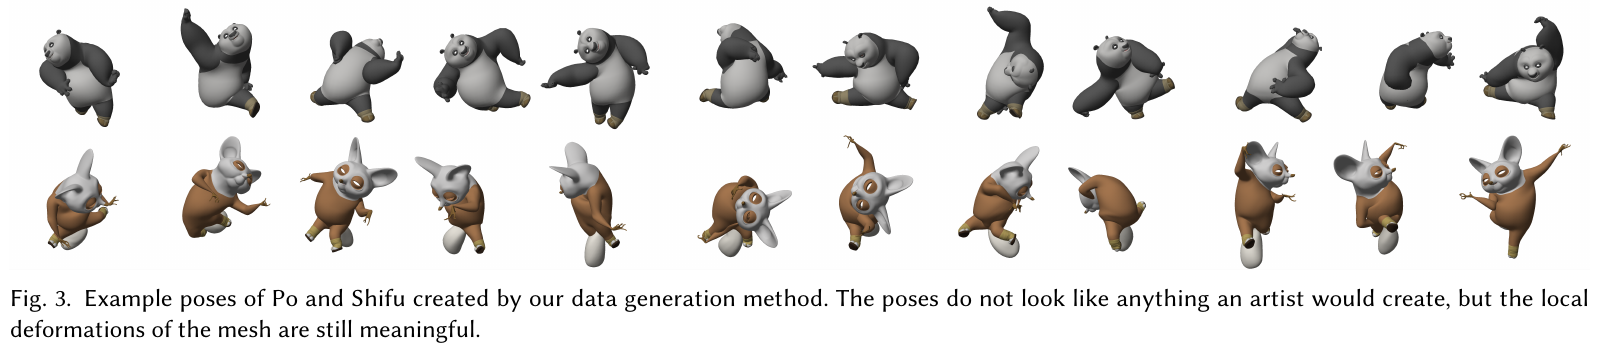
\includegraphics[width=\textwidth]{img/dataset}
    };
  }
\end{frame}

\begin{frame}
  \TikzDraw {
    \node at (0, 0) {\Huge{Results}};
  }
\end{frame}

\begin{frame}
  \TikzDraw {
    \node at (0, 2.5) { 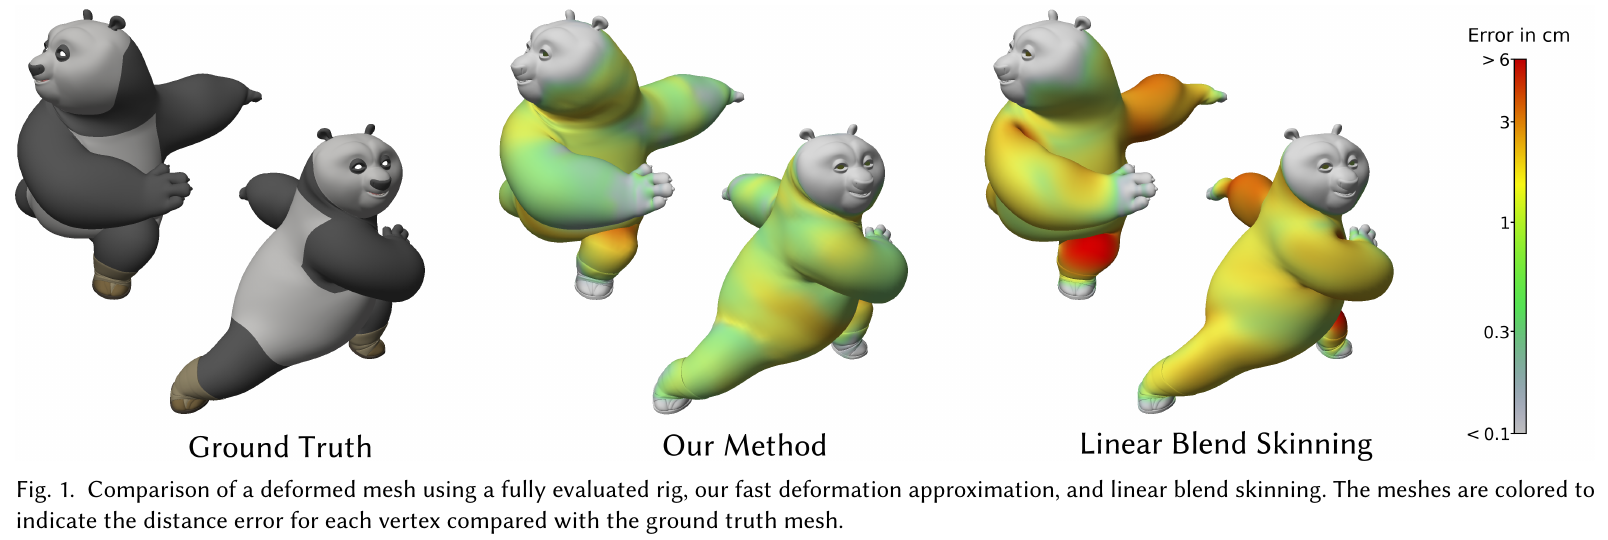
\includegraphics[width=\textwidth]{img/teaser} };
    \node at (-3, -1.5) {
      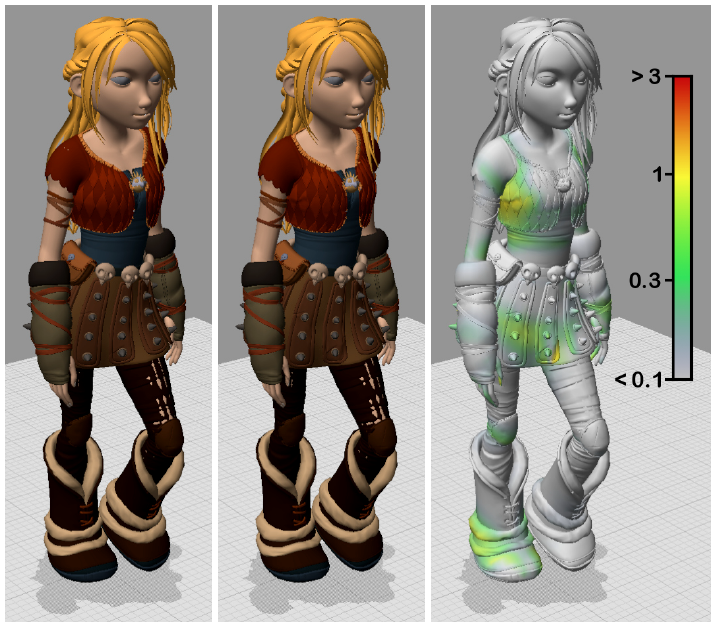
\includegraphics[width=0.4\textwidth]{img/girl}
    };
    \node at (2.5, -1.5) {
      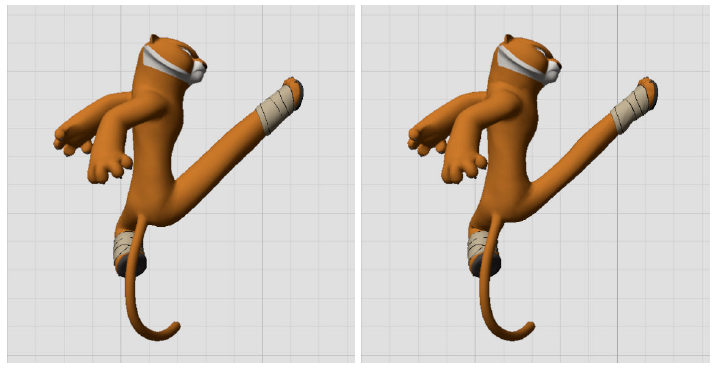
\includegraphics[width=0.6\textwidth]{img/tiger}
    };
  }
\end{frame}

\begin{frame}
  \frametitle{Comparison}
  \TikzDraw {
    \node at (-3, 0) {
      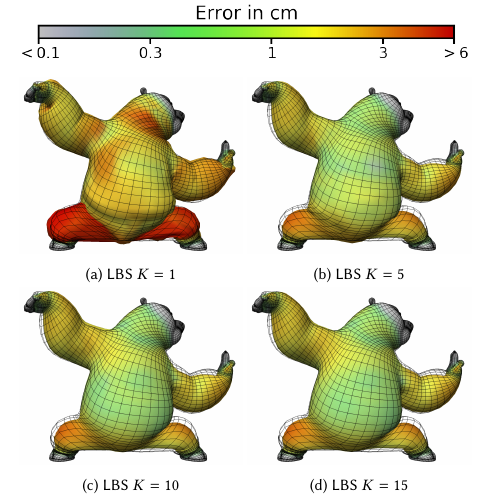
\includegraphics[width=0.5\textwidth]{img/comparison_u}
    };
    \node at (3, -0.36) {
      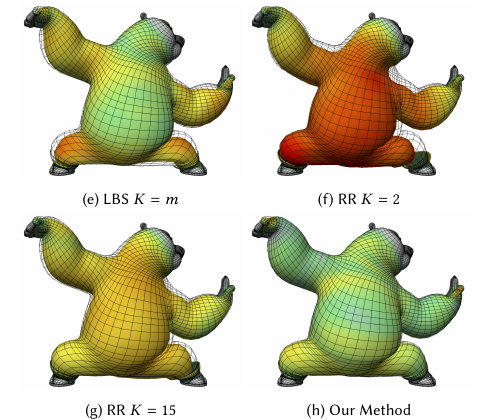
\includegraphics[width=0.5\textwidth]{img/comparison_b}
    };
  }
\end{frame}

\begin{frame}
  \frametitle{Comparison}
  \begin{figure}
    \centering
    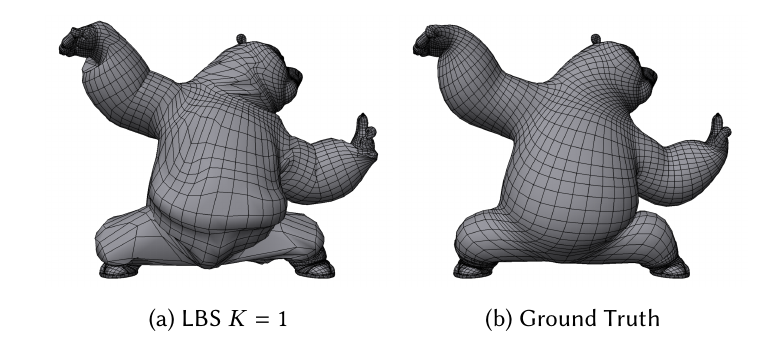
\includegraphics[width=\textwidth]{img/mesh_comp}
  \end{figure}
\end{frame}

\begin{frame}
  \frametitle{Comparison}
  \begin{figure}
    \centering
    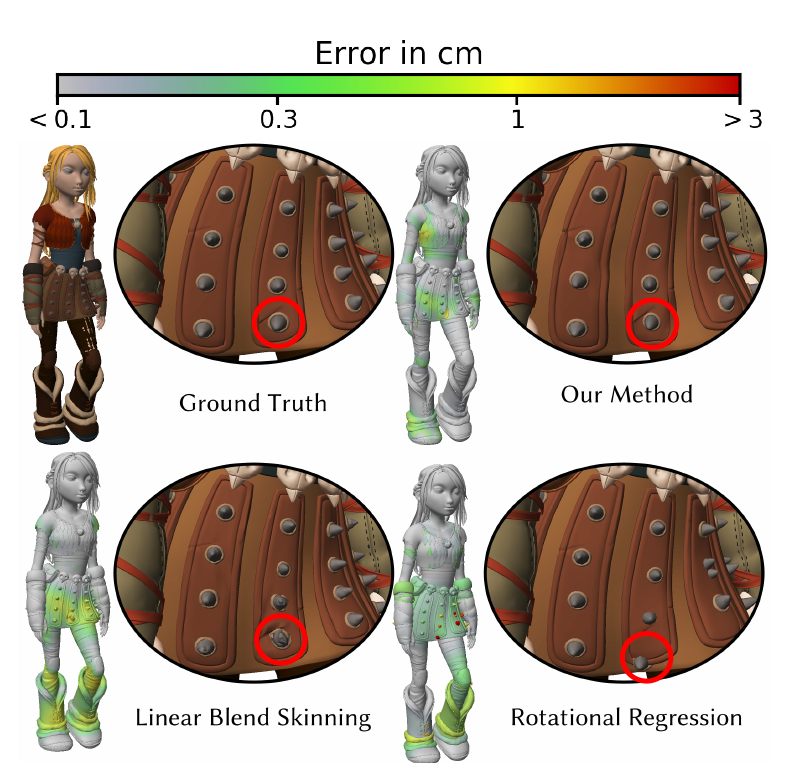
\includegraphics[width=0.7\textwidth]{img/details}
  \end{figure}
\end{frame}

\begin{frame}
  \frametitle{Performance}
  \TikzDraw {
    \node at (0, 1.5) {
      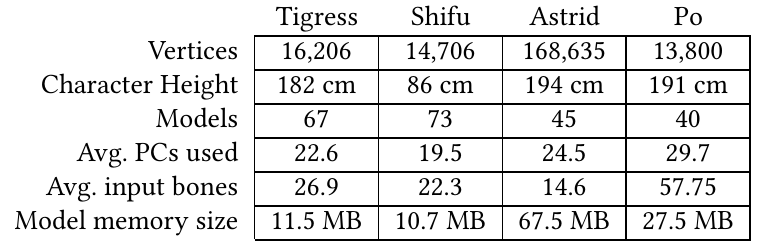
\includegraphics[width=\textwidth]{img/data_info}
    };
    \node at (0, -2) {
      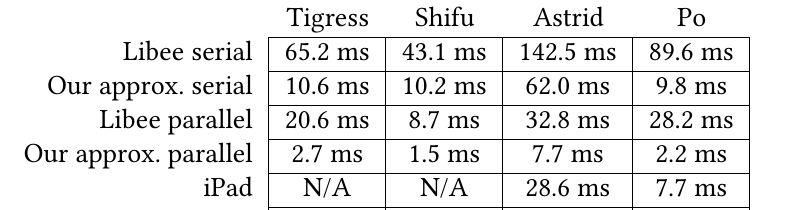
\includegraphics[width=1.05\textwidth]{img/performance}
    };
    \draw[red, thick] (-5.5, -3.6) rectangle (5.4, -2.4);
  }
\end{frame}

\begin{frame} 
  \TikzDraw {
    \node at (0, 0.5) {\Huge{Thanks!}};
  }
  %\gridlines
\end{frame}

\end{document}
